\documentclass[MTech]{iitmdiss}
\usepackage{times}
\usepackage{epsf}
\usepackage{threeparttable}
\usepackage{setspace}
\usepackage{amsmath}
\usepackage{bm}
\usepackage{amsthm}
\usepackage{txfonts,pxfonts,amsfonts}
\usepackage{epsfig}	
\usepackage{caption}
\usepackage{subfig}
\usepackage{subcaption}
\usepackage{listings}
\usepackage{epstopdf}
%\usepackage[dvips]{graphicx}
\usepackage{graphicx}
\usepackage{comment}
%\usepackage{pstricks,pst-node,pst-tree,pstricks-add}
% \usepackage[square,numbers,sort]{natbib}
%\usepackage{biblatex}
\usepackage[square]{natbib}
\usepackage{hyperref}
%\usepackage[hypertex]{hyperref} % hyperlinks for references.
% \usepackage{algorithmic}
\usepackage{algorithm}
\usepackage{algpseudocode}
\usepackage{color}
% \usepackage[demo]{graphicx}


\newcommand\blfootnote[1]{%
  \begingroup
  \renewcommand\thefootnote{}\footnote{#1}%
  \addtocounter{footnote}{-1}%
  \endgroup
}
%\include{commands}

% Strut macros for skipping spaces above and below text in tables. 
\def\abovestrut#1{\rule[0in]{0in}{#1}\ignorespaces}
\def\belowstrut#1{\rule[-#1]{0in}{#1}\ignorespaces}

\def\abovespace{\abovestrut{0.20in }}
\def\aroundspace{\abovestrut{0.20in}\belowstrut{0.10in}}
\def\belowspace{\belowstrut{0.10in}}
%%%%%%%%%%%%%%%%%%%%%%%%%
\def\thesistitle{Parallel Subgraph Isomorphism}
\def\thesisauthor{Shreyas Phanse}

\begin{document}
\bibliographystyle{iitm}
%%%%%%%%%%%%%%%%%%%%%%%%%%%%%%%%%%%%%%%%%%%%%%%%%%%%%%%%%%%%%%%%%%%%%% 
% Title page

\title{\thesistitle}
\author{\thesisauthor}

\date{April 2018}
\department{Computer Science and Engineering}

%\nocite{*}
\begin{singlespace}
\maketitle 
\end{singlespace} 



%%%%%%%%%%%%%%%%%%%%%%%%%%%%%%%%%%%%%%%%%%%%%%%%%%%%%%%%%%%%%%%%%%%%%%
% Certificate
\certificate
\vspace*{0.5in}
\noindent This is to certify that the thesis entitled {\bf {\thesistitle}}, 
submitted by {\bf {\thesisauthor}}, to the Indian Institute of Technology, 
Madras, for the award of the degree of {\bf Master of Technology}, 
is a bonafide record of the research work carried out by him under my
supervision. The contents of this thesis, in full or in parts, have not been
submitted to any other Institute or University for the award of any degree or diploma.
\vspace*{1.4in}
\hspace*{-0.25in}
\begin{singlespace}
\noindent {\bf Dr.~Rupesh~~Nasre} \\
\noindent Project Guide \\ 
\noindent Asst. Professor \\
\noindent Dept. of Computer Science and Engineering\\
\noindent IIT-Madras, 600 036 \\
\end{singlespace}
\vspace*{0.20in}
\noindent Place: Chennai\\ 
Date: 23 April 2018


%%%%%%%%%%%%%%%%%%%%%%%%%%%%%%%%%%%%%%%%%%%%%%%%%%%%%%%%%%%%%%%%%%%%%%
% Acknowledgements
\acknowledgements
My foremost gratitude and respects to my guide Dr. Rupesh Nasre for his guidance, motivation and moral support in my execution of this project work. His constant motivation for me towards the project helped me throughout the project.

I also thank my friends Mahesh Magar, Maniraja Pedaprolu, Ganesh k. who supported me throughout the project and constantly encouraged me to work harder. I thank my parents and my sister to help my balance my work my constantly motivating me.
%%%%%%%%%%%%%%%%%%%%%%%%%%%%%%%%%%%%%%%%%%%%%%%%%%%%%%%%%%%%%%%%%%%%%%

%%%%%%%%%%%%%%%%%%%%%%%%%%%%%%%%%%%%%%%%%%%%%%%%%%%%%%%%%%%%%%%%%%%%%%
% Abstract
\abstract


\vspace*{24pt}

Subgraph isomorphism is used in many real world problems such as chemical compounds, social networks, and biological structures. Many real applications in bio-informatics, chemistry, and software engineering require efficient and effective management of graph structured data.

One of most important graph queries in graph databases is the subgraph isomorphism query. That is, given a query q and a data graph g, find all embeddings (matches) of q in g. This problem is NP-hard. Various popular algorithms that have tried to solve the problem in reasonable amount of time.

With the development of GPUs and the number of cores, there has been a huge increment in amount of parallelism achieved and therefore increasing the speed up and performance of algorithm. In this project, we have tried to parallelise subgraph isomorphism algorithm and compare it with the sequential implementation. We have studied the scenarios where each of these implementations outperform each other

\pagebreak
%%%%%%%%%%%%%%%%%%%%%%%%%%%%%%%%%%%%%%%%%%%%%%%%%%%%%%%%%%%%%%%%%
% Table of contents etc.
\begin{singlespace}
\tableofcontents
\thispagestyle{empty}
\listoftables
\addcontentsline{toc}{chapter}{LIST OF TABLES}
\listoffigures
\addcontentsline{toc}{chapter}{LIST OF FIGURES}
\end{singlespace}
%%%%%%%%%%%%%%%%%%%%%%%%%%%%%%%%%%%%%%%%%%%%%%%%%%%%%%%%%%%%%%%%%%%%%%
% Abbreviations
\include{parts/abbreviation}
\pagenumbering{arabic}

%%%%%%%%%%%%%%%%%%%%%%%%%%%%%%%%%%%%%%%%%%%%%%%%%%
 % Chapters.
\chapter{INTRODUCTION}
\label{chap:intro}


\section{Motivation}
A large number of real world scenarios can be modelled as graphs and a number of real world problems can be solved by using graph algorithms. For example, shortest distance between two cities can be found using the Dijkstra’s shortest path algorithm by modelling the cities and the roads connecting them as graphs. Similarly, other problems such as relation between people, chemical compounds, DNA sequences etc. can be modelled as graphs and many complex problems related to them can be solved using various graph algorithms. 

One of the most important type of graph problem is Subgraph isomorphism. In real world problems which are modelled as graphs, subgraph isomorphism is an important problem. Since this problem is NP-hard, it is not an easy task to find solutions for large graphs in a small amount of time. however, Recent works have been able to solve the problem in quite a reasonable amount of time on specific real-world datasets. Because of numerous applications of the problem in many data mining and pattern matching fields, the problem has been studied through years and different methods have been proposed over time. Some of the state-of-the-art techniques for the same have been studied and discussed in upcoming sections. In recent years, with the development of parallel programming and GPUs, massive speedups have been achieved on execution of various computing tasks. Our objective is to exploit this to obtain even faster query outputs for large graphs.

\section{Problem Statement}

\textbf{Graph:}\\
A graph $g$ is defined as a 3-tuple $(V,E,L)$ where $V$ is the set of vertices, $E(\subseteq V \times V)$ is the set of edges, and $L$ is a label function that maps a vertex to a set of labels. Without loss of generality, all subgraph isomorphism algorithms can be easily extended to handle graphs whose edges have labels.\\
\textbf{Subgraph Isomorphism:}\\
A graph $q$ = $(V, E,L)$ is isomorphic to a subgraph of a data graph $g = (V', E', L')$ if there is an injection (or an embedding) $M : V \rightarrow V$ such that, $\forall u \in V $, $L(u) \subseteq L' (M(u))$, and $\forall (u_i, u_j) \in E$, $(M(u_i), M(u_j)) \in E'$. Such a subgraph is also called an embedding.\\
Now, the subgraph isomorphism problem is defined as follows: “Given a query graph q and a data graph g, find all distinct embeddings of q in g.” This is explained by the following example.

\begin{figure}[h]
\centering 
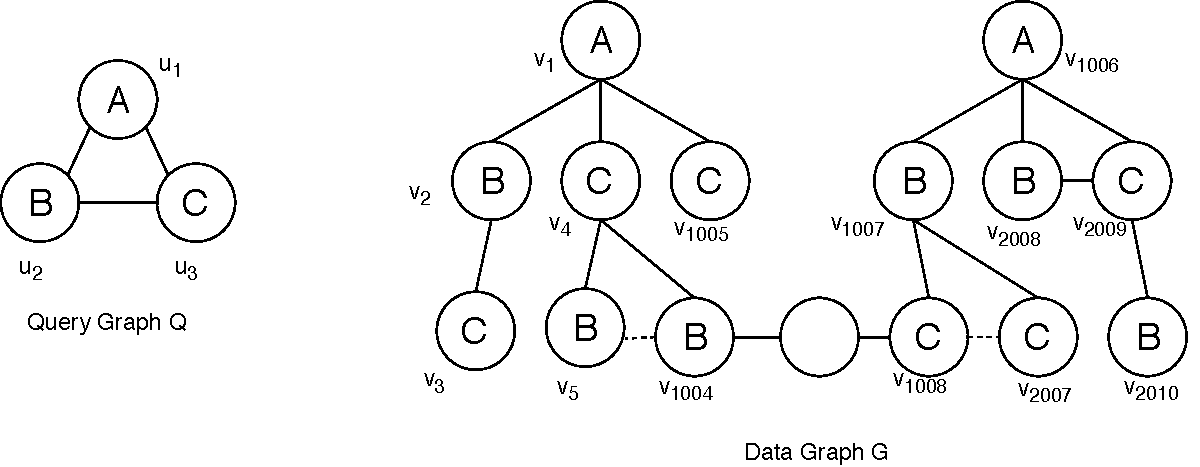
\includegraphics[width=\columnwidth]{images/graph.pdf}
\caption[Subgraph Isomorphism]{A query graph $q$ and a data graph $g$} % The text in the square bracket is the caption for the list of figures while the text in the curly brackets is the figure caption
\label{fig:gallery} 
\end{figure}

For the above query graph, the data subgraph {$v_{1006}, v_{2008}, v_{2009}$} is isomorphic to the query graph and hence is a match. There is no other match for the given query graph in the data graph.

\section{Data Representation}

In the implementation, graphs are represented as compressed sparse rows(CSR). The CSR representation of a matrix consists of several one dimensional arrays. The number of arrays depends upon the information carried by the matrix. For example, consider the adjacency matrix of a labelled graph with 9 vertices as shown in the figure below. For this graph, the CSR representation will contain 3 vectors (1-d arrays), namely IA, JA and LA, which are defined as:

IA is an array of size rows(M) + 1 which is recursively defined as:
\begin{itemize}
    \item $IA[0] = 0$
    \item $IA[i]$ = $IA[i - 1]$ + number of non zero entries in $i - 1^{th}$ row of M
\end{itemize}

JA is an array of size equal to value last element of IA i.e. the number of edges in the graph. The entries of JA are the column numbers of all the non zero entries of from left to right row-wise.

LA is an array of size rows(M). It contains the labels of all the nodes in order. For the graph in figure 1.2, the matrix M and CSR representation are given.

\begin{figure}[h]
\centering 
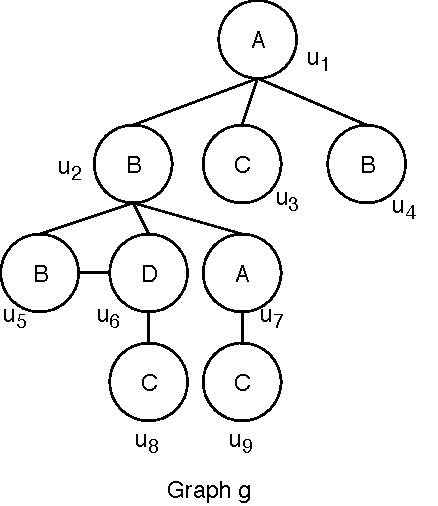
\includegraphics[scale = 0.8]{images/csr.pdf}
\caption[Graph representation]{Graph representation : graph $g$} % The text in the square bracket is the caption for the list of figures while the text in the curly brackets is the figure caption
\label{fig:gallery} 
\end{figure}

\[
    M =
    \begin{bmatrix}
        0 & 1 & 1 & 1 & 0 & 0 & 0 & 0 & 0\\
        1 & 0 & 0 & 0 & 1 & 1 & 1 & 0 & 0\\
        1 & 0 & 0 & 0 & 0 & 0 & 0 & 0 & 0\\
        1 & 0 & 0 & 0 & 0 & 0 & 0 & 0 & 0\\
        0 & 1 & 0 & 0 & 0 & 1 & 0 & 0 & 0\\
        0 & 1 & 0 & 0 & 1 & 0 & 0 & 1 & 0\\
        0 & 1 & 0 & 0 & 0 & 0 & 0 & 0 & 1\\
        0 & 0 & 0 & 0 & 0 & 1 & 0 & 0 & 0\\
        0 & 0 & 0 & 0 & 0 & 0 & 1 & 0 & 0\\
    \end{bmatrix}
\]
\\
\[
    IA = 
    \begin{bmatrix}
        0 & 3 & 7 & 8 & 9 & 11 & 14 & 16 & 17 & 18
    \end{bmatrix}
\] 
\[
    JA =
    \begin{bmatrix}
        1 & 2 & 3 & 0 & 4 & 5 & 6 & 0 & 0 & \dots
    \end{bmatrix}
\]
\[
    LA =
    \begin{bmatrix}
        A & B & C & B & B & D & A & C & C
    \end{bmatrix}
\]


\section{CUDA Architecture}

Figure 1.3 gives an overview of modern day GPU architecture. \cite{book} has been referred for CUDA related concepts. CUDA enabled GPU is made up of number of highly threaded streaming microprocessors. In the figure, there are 2 streaming multiprocessors in each building block. Each of these streaming microprocessors is itself made up of streaming processors (6 SPs per SM in figure 2). These steaming processors share control logic and instruction cache.The global memory is made of DRAM and has very high bandwidth. Although the GPU global memory has higher latency as compared to the CPU RAM, highly parallel applications can compensate for the latency as it has higher bandwidth resulting in superior execution time.

\begin{figure}[h]
\centering 
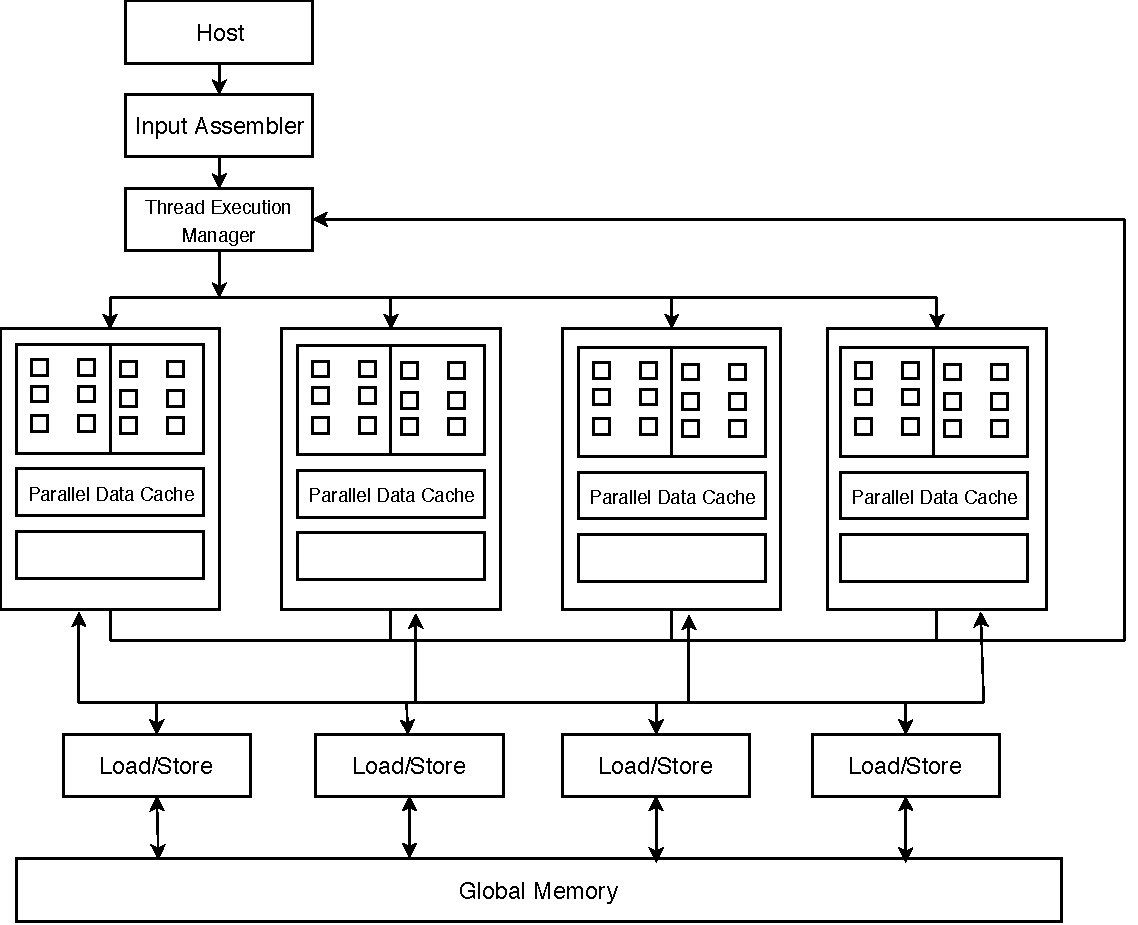
\includegraphics[width=\columnwidth]{images/gpu.pdf} 
\caption[CUDA architecture]{CUDA enabled GPU architecture} % The text in the square bracket is the caption for the list of figures while the text in the curly brackets is the figure caption
\label{fig:gallery} 
\end{figure}

\section{Organization of the Thesis}
Chapter \ref{chap:lit} discusses the previous works in this area and related concepts. In Chapter 3, the parallel implementation is discussed with example. Chapter 4 discusses the comparative study of performances of the sequential and the parallel implementations. The datasets on with the study is done are also explained in this section. Chapter 5 concludes the work with analysis and proposes future work and optimizations that can be done to improve the speedup.
\chapter{LITERATURE SURVEY}
\label{chap:lit}

This section discusses various state-of-the-art algorithms that have been developed. Ideas from these algorithms have been used in implementation of the parallel algorithm.

\section{Generic Algorithm}

The Generic Algorithm is template that is used most of the algorithms discussed in upcoming sections. Most of the popular algorithms are variations of the generic algorithm. It must be noted that the efficiency of algorithms depends on the heuristics used for pruning the candidate list and selecting the order of vertices that are to be matched. The Generic Algorithm uses backtracking for finding the solutions. If we find out that solution cannot be achieved from a call, we end that call and proceed to the next.

\begin{algorithm}

\caption{\textsc{GenericAlgo}}\label{euclid}

\begin{algorithmic}[1]

%\textbf{Input:} Data graph g, Query graph q.\\

%\textbf{Output:} all subgraph isomorphisms of q in g.

\State $M \gets \emptyset$

\ForAll{$u \in V(q)$}

\State $C(u) \gets \textsc{FilterCandidates}$

\If{$c = \emptyset$}

\State \textbf{return}

\EndIf

\EndFor

\State $\textsc{SubgraphSearch}$ 

\Procedure{$\textsc{SubgraphSearch}$}{}

\If{$|M| = |V(q)|$}

    \State \textbf{report} M

    \Else

    \State $u \gets \textsc{NextQueryVertex}(..)$

    \State $C_R \gets \textsc{RefineCandidates}(...)$

    \ForAll{$V \in C_R$ such that v is not yet matched}

        \If{\textsc{IsJoinable}}

            \State \textsc{UpdateState}

        \EndIf

    \EndFor

\EndIf

\EndProcedure

\end{algorithmic}

\end{algorithm}

Algorithm 1 shows a generic subgraph isomorphism algorithm, \textsc{GenericAlgo}. Its inputs are a query graph q and a data graph g, and its output is a set of subgraph isomorphisms (or embeddings) of q in g. Here, to represent an embedding, we use a list M of pairs of a query vertex and a corresponding data vertex. The specific implementations of these procedures have been discussed in the respective subsections.

\section{Ullmann Algorithm}

Ulmann Algorithm was proposed in \cite{ullmann}. It exploits the template mentioned in Generic algorithm in the following way.\\
\\
\textsc{FilterCandidates:} \textsc{FilterCandidates} returns a set that contains the vertices whose label set is a subset of label set of $u$. For example, in figure $1$, it will return candidates of $u_1$ as \{$v_1, v_{1006}$\}\\
\\
\textsc{NextQueryVertex:} Returns the next data vertex that is to be checked. Ullmann Algorithm takes the vertices the the same order in which they appear in the input. Hence the result of this Algorithm highly depends on the input order. This issue is discussed in the next subsection.\\
\\
\textsc{RefineCandidates:} Prunes out all candidate vertices that have a smaller degree than u. In our running example, $v_{1005}$ will be pruned out as a candidate for $u_3$ because it has degree less than that of $u_3$ and hence can never map to it.\\
\\
\textsc{IsJoinable:} For all the vertices that have been matched, the \textsc{IsJoinable} checks whether there is a data edge corresponding to an edge in the query graph. In our running example, \{$u_1, u_2, u_3$\} will be matched to \{$v_1, v_2, v_3$\}. The \textsc{IsJoinable} procedure will check if there are corresponding edges between these matches. Since the edge between $v_2$ and $v_4$ is absent, the \textsc{IsJoinable} procedure will return false.

\section{VF2 algorithm}

This algorithm was published by \cite{vf2}. Following is the implementation of the algorithm in brief.

\textsc{NextQueryVertex:} VF2 Algorithm does not process data vertices in the order of input. Rather, from the start vertex, it returns the vertex which is a neighbour to the vertex (DFS like fashion). However, it does not use any particular method for selecting a neighbour. Hence, It does not exploit any property of the data/query graph.\\
\\
\textsc{RefineCandidates:} VF2 uses the following pruning
rules to prune out data vertex candidates:
\begin{enumerate}
    \item If there is vertex $v$ in the candidate list of a vertex $u$ that is not  connected to an already matched vertex, it is pruned out of the candidate list.
    \item If there is vertex $v$ in the candidate list of a vertex $u$, then the number of unmatched vertices connected to $v$ must be larger than those of $u$.
\end{enumerate}

\section{QuickSI Algorithm}

This algorithm was proposed in \cite{quicksi}.\\
\textsc{NextQueryVertex:} The QuickSI Algorithm exploits properties of the data and query graphs in order to prune candidate list more quickly and get better matching sequence compared to the previously discussed ones. It preprocesses the data graphs for increased efficiency by maintaining 'score' for each vertex. Scores are calculated by assigning weights to each vertex in accordance to frequency of its label and degree of the vertex. Then the algorithm selects the vertices in the order in which they appear in the minimum spanning tree. This heuristic is very efficient as the low label frequency vertices have lower probability of getting a candidate and hence will get pruned earlier. In most of the cases, QuickSI gives a better result than Ullmann and VF2 algorithm when run sequentially.


\section{Turbo\_iso Algorithm}

\begin{algorithm}
\caption{\textsc{$Turbo_{ISO}(g,q)$}}\label{euclid}
\begin{algorithmic}[1]
%\textbf{Input:} Data graph g, Query graph q.\\
%\textbf{Output:} all subgraph isomorphisms of q in g.
\State $u_s \gets \textsc{ChooseStartQueryVertex(q,g)}$
\State $q' \gets \textsc{ReWriteToNECTree}(q,u_s)$ // q': NEC Tree
\ForAll{$v_s$ in {$v|(v \in V(g))$ and $(L(u_s) \subseteq L(v))$}}
    \If{$\textsc{ExploreCR}(u'_s,{v_s},CR)=FAIL$}
        \State \textbf{continue}
    \EndIf
    \State order = $\textsc{DetermineMatchingOrder}(q',CR)$
    \State $\textsc{UpdateState}(M,F,{us},{vs})$
    \State $\textsc{SubGraphSearch}(g,q',q,order)$
    \State $\textsc{RestoreState}(M,F,{u_s},{v_s})$
\EndFor
\end{algorithmic}
\end{algorithm}

\begin{figure}[H]
\centering 
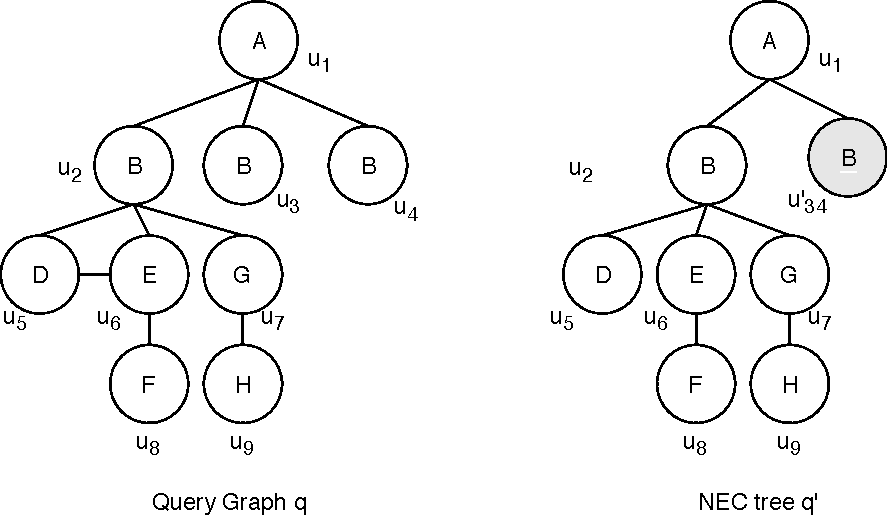
\includegraphics[width=\textwidth]{images/nec.pdf} 
\caption[Query graph and NEC Tree]{A query graph and its corresponding NEC Tree} % The text in the square bracket is the caption for the list of figures while the text in the curly brackets is the figure caption
\label{fig:gallery} 
\end{figure}


This algorithm was proposed in \cite{turbo}. $Turbo_{ISO}$ uses the concept of Neighbourhood Equivalence Class (NEC). Two vertices are said to be in an NEC if:
\begin{enumerate}
    \item They have same labels.
    \item The have exactly same subtrees (considering undirected graphs).
\end{enumerate}
Figure 2.1 shows a query graph and it's equivalent NEC tree.
In figure 2, $u_2$ and $u_3$ follow the above 2 rules and hence belong to the same NEC ($u^{'}_{2,3}$).
Matching time can be reduced using this concept as number of vertices that are to be matched will be reduced. Using NEC tree, we can reduce the number of call by huge margin as calls for vertices that are identically matching will be made only once. However, in order to generate all the matches, we will have to permute all the combinations for every NEC.
\chapter{Implementation}
\label{chap:dpp}

\section{Data Pre-processing}
In this section, we discuss various attempts made to reduce the search space and unnecessary recursion calls to save time and space. Following techniques have been used:

\subsection{Candidate List Generation}

\begin{frame}{}
\begin{algorithm}
\caption{\textsc{getCandidates}}\label{euclid}

\textbf{Input:} Data graph g, Query graph q, Data vertex v.\\
\textbf{Output:} Candidate set of all $u \in V(q)$

\begin{algorithmic}[1]
\State $Candidate \gets \emptyset$\\
\Comment{\textcolor{green}{For all $v \in V(g)$, we launch a thread. Each thread performs the following operation}}

\ForAll{$u \in V(q)$}
\If{$degree(v) > degree(u)$ \&\& $L(u) = L(v)$}
    \State \textcolor{blue}{index = atomicIncrement(numCandidates(u))}
    \State \textcolor{blue}{$Candidate(u, index) \gets v$}
\EndIf
\EndFor
\State \textbf{return} $Candidate$
\end{algorithmic}
\end{algorithm}
\end{frame}

This process helps to reduce the search space by identifying those vertices of data graph which can possibly be a match for any vertex of query graph. For a particular vertex u of a query graph, A vertex v of data graph is said to be a candidate iff:
\begin{itemize}
    \item $|v| \geq |u|$
    \item $L(v)=L(u)$
\end{itemize}

\begin{figure}[h!]
\begin{center}
        \centering
        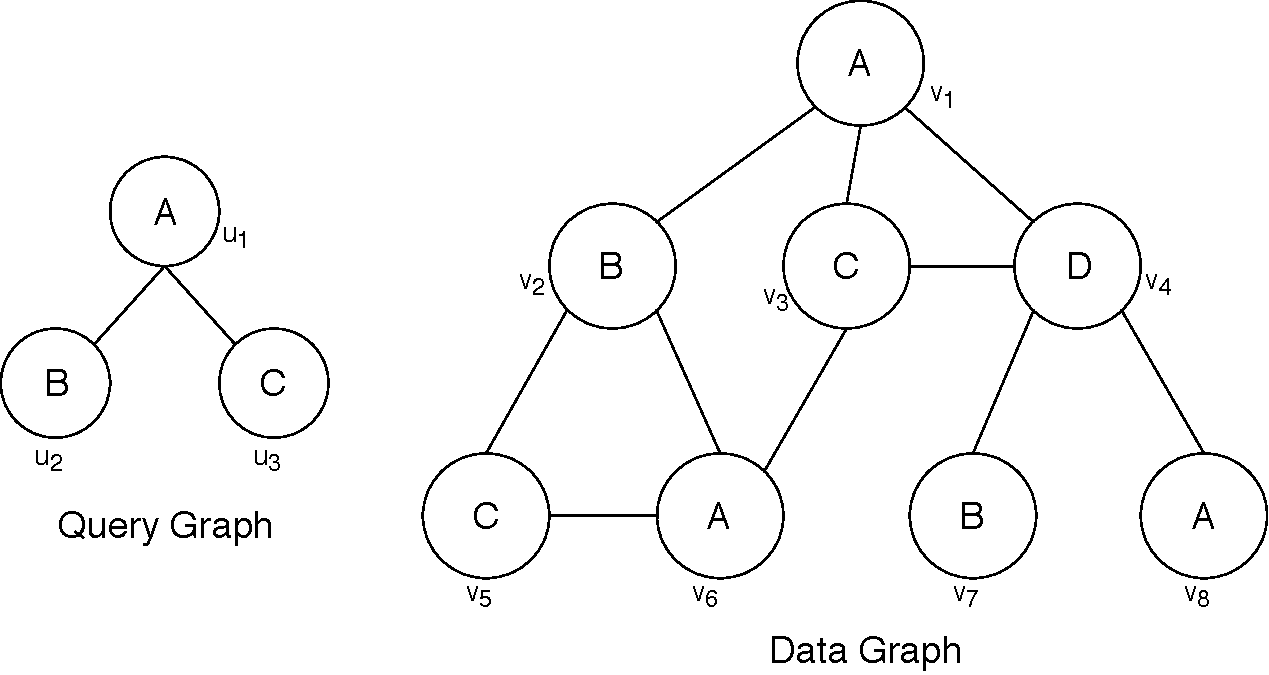
\includegraphics[width=\textwidth]{images/Implementation.pdf}
        \caption{Data Graph g and Query Graph q}
        \label{fig:flowchart}
\end{center}
\end{figure}

Consider the data graph and query graph as shown. As per the definition, the candidate list of $u_1$ = \{$v_1, v_6$\}, candidate list of $u_2$ = \{$v_2, v_7$\} and $u_3$ = \{$v_3, v_5$\}.

In the parallel implementation of the method, we launch a thread for every vertex v of data graph. Each thread then finds all the query vertices of which v can be a candidate of. Since there is a data race between each thread to add a vertex $v \in V(d)$ to the candidate set of vertex $u \in V(q)$, atomicInc is used to prevent any data hazard due to the race. The numCandidate(u) returns the number of candidates of a vertex $u \in V(q)$ found so far.

\section{Query vertex ordering}

The order in which \textsc{FindMatch} processes the query vertex also determines the time of execution of algorithm. In order to have an efficient query vertex ordering, we suggest the following score function given to each query vertex:
\[
score(u) = N(L(u), g)/|v|
\]
where N(L(u), g) is the number of vertices in the data graph with the same label as that of u. The query vertices are then sorted in ascending order of their score. For e.g. for the graphs in figure 3.1, the order of query vertices will be $u_1$-$u_2$-$u_3$ with scores of 1.5, 2 and 2. The idea behind this scoring function is that higher the degree of a node, the more likely it is to get pruned while searching for a match. Inversely, the lesser the number of vertices in data graph with the same label as that of u, the more likely it will get pruned faster. However this may not always be the best choice.

\section{Algorithm}

In the parallel implementation of the Algorithm, first, we obtain all the candidate set of vertices of the query graph. Then we obtain the order in which we are to process the query vertices. These processes have been discussed in the previous section.

In the parallel implementation of \textsc{findMatch}, we select the first query vertex that is to be processed. For each candidate of the query vertex, we launch a thread that calls \textsc{subgraphSearch}. The \textsc{subgraphSearch} procedure recursively checks for the candidates of the next query vertex that is to processed. If the candidate is joinable, i.e. the corresponding edges between the vertices in M and the corresponding vertices in q exist, then candidate is added to M.

For example, in the graph shown in figure 3.2, vertex $u_1$ is selected and two threads are launched which search for the match from vertices $v_6$ and vertex $v_1$ respectively. The threads then check for the candidates of vertices to follow. Say $thread\_0$  is launched corresponding to the vertex $v_1$, it will check for the candidates of the vertex $u_2$. Since the corresponding edges between the vertices \{$u_1$, $u_2$\} and \{$v_1$, $v_2$\} exist,  vertex $v_2$ is added to M and the state is updated. Similarly, since the corresponding edges between the vertices \{$u_1$, $u_2$\} and \{$v_1$, $v_7$\} do not exist, the vertex $v_7$ is discarded. Next, candidates of vertex $u_3$ are checked. In the graph, since the vertices \{$u_1$, $u_2$, $u_3$\} and \{$v_1$, $v_2$, $v_3$\} have the corresponding edges matched, the procedure \textsc{SubgraphSearch} reports it as a match. Since corresponding edges between \{$u_1$, $u_2$, $u_3$\} and \{$v_1$, $v_2$, $v_5$\} do not match, $v_5$ is discarded and the function returns.

\begin{figure}[]
\begin{center}
        \centering
        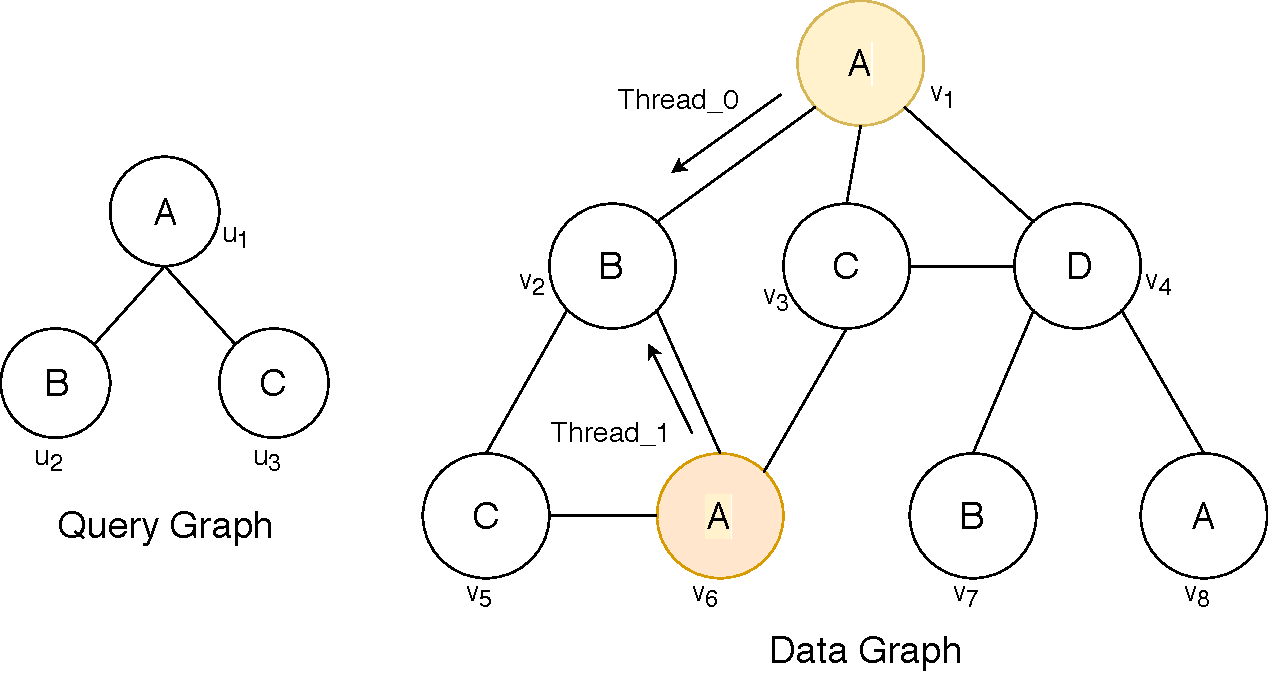
\includegraphics[width=\textwidth]{images/Implementation_thread.pdf}
        \caption{\textsc{SubgraphSearch}}
        \label{fig:flowchart}
\end{center}
\end{figure}

Similarly, say $thread_1$ is launched corresponding to the vertex $v_6$. Similar procedure is performed i.e. vertex $v_2$ is added to M. In the next recursive call, both vertices $v_3$ and $v_5$ report a match. While the vertex $v_7$ is discarded because the corresponding edges do not match. Hence the the algorithm reports the match \{$v_1$, $v_2$, $v_3$\} (reported by thread\_0), \{$v_6$, $v_2$, $v_5$\} and \{$v_6$, $v_2$, $v_3$\} (reported by thread\_1).

\begin{frame}{}
    \begin{algorithm}
\caption{\textsc{FindMatch}}\label{euclid}
\textbf{Input:} Data graph g, Query graph q, Candidate set C, Order of processing Query vertices\\
\textbf{Output:} all subgraph isomorphisms of q in g.

\begin{algorithmic}[1]
\State $M \gets \emptyset$
\State $C \gets \textsc{getCandidates}$
\State $u \gets \textsc{NextQueryVertex}$
\State \textsc{UpdateState(M, u, v...)}\\
\Comment{\textcolor{green}{For each $u' \in C(u)$, we launch a thread. each of which performs following operation}}
\State $\textsc{SubgraphSearch}(u^{'}, q, g, M,...)$ 
\Procedure{$\textsc{SubgraphSearch}(u, q, g, M,...)$}{}[0]
\If{$|M| = |V(q)|$}
    \State \textsc{\textcolor{blue}{lock()}}
    \State \textbf{report} M
    \State \textsc{\textcolor{blue}{unlock()}}
    \Else
    \State $u^{'} \gets \textsc{NextQueryVertex}$
    
    \ForAll{$v \in C(u^{'})$}
        
        \If{\textsc{$\sim$ IsVisited(v)}}
    
            \If{\textsc{IsJoinable}(q, g, M, u, v)}
                    \State \textsc{UpdateState(M, u, v...)}
                    \State $\textsc{SubgraphSearch}(u, q, g, M,...)$
            \Else
                    \State RestoreState(M, q, g, )
                    \State \textbf{return}
            \EndIf
        \EndIf

    \EndFor
    
\EndIf
\EndProcedure{}
\end{algorithmic}
\end{algorithm}
\end{frame}


\section{Challenges}

\subsection{Recursive Implementation}

Initially, the algorithm was implemented using recursion. However, since CUDA supports recursive implementation upto 24 levels, the algorithm did not work for query graph of size 8 vertices. To overcome this problem, the recursive procedure is implemented by maintaining stack. Following pseudocode shows stack implementation of \textsc{SubgraphSearch}


\begin{frame}{}
    \begin{algorithm}
\caption{\textsc{SubgraphSearch\_Stack}}\label{euclid}
% \textbf{Input:} Data graph g, Query graph q, Candidate set C, Order of processing Query vertices\\
% \textbf{Output:} all subgraph isomorphisms of q in g.
\begin{algorithmic}[1]
\State $M \gets \emptyset$
\State $C \gets \textsc{getCandidates}$
\State $u \gets \textsc{NextQueryVertex}$
\State \textsc{push} $u$
\While{$\sim$ \textsc{stackEmpty}}
    \State \textsc{pop}
    
    \If{$|M| = |V(q)|$}
        \State \textsc{\textcolor{blue}{lock()}}
        \State \textbf{report} M
        \State \textsc{\textcolor{blue}{unlock()}}
        
    \Else
        \If{\textsc{$\sim$ IsVisited(v)}}
            \If{\textsc{IsJoinable}(q, g, M, u, v)}
                \State \textsc{UpdateState(M, u, v...)}
                \State \textsc{push} next candidate of current query vertex
                \State \textsc{push} a candidate of next query vertex
            \EndIf
            
        \Else
            \State \textsc{push} $u$
        \EndIf
    \EndIf
\EndWhile

\end{algorithmic}
\end{algorithm}
\end{frame}




\subsection{Exponential Complexity}

Because of the exponential complexity of the algorithm, a number of implementational challenges were faced. One of them being the use of dynamic parallelism. Since at each step number of calls increase exponentially, so does the number of threads. Hence dynamic parallelism is not used for implementing the algorithm.

\chapter{Experiments and Results}
\label{chap:exp}
 
\section{Datasets}

The parallel implementation of Subgraph Isomorphism Algorithm has been compared to sequential implementation of VF2 algorithm on various real world datasets. Following is a brief overview of the datasets that have been used to perform experiments.

\begin{table}[h!]
  \begin{center}
    \caption{Datasets}
    \label{tab:table1}
    \begin{tabular}{l||l|l} % <-- Alignments: 1st column left, 2nd middle and 3rd right, with vertical lines in between
      \textbf{Dataset} & \textbf{Vertices} & \textbf{Edges}\\
      \hline
      Jazz musicians & 198 & 2742\\
      Facebook (NIPS) & 2888 & 2981\\
      	U. Rovira i Virgili & 1133 & 5451\\
      	Hamsterster friendships & 1858 & 12534\\
      	US power grid & 4941 & 6594\\
      	Chicago transporation & 1467 & 1298
    \end{tabular}
  \end{center}
\end{table}

For these datasets, random connected query graphs are generated to run the algorithm. To generate labelled graphs, labels are randomly allotted to the vertices of the data and query graphs.

\section{Dataset: Jazz Musicians}

The Jazz Musicians dataset (\cite{jazz}) represents a network of musicians where each edge represents that the corresponding musicians have played together at some point. This is a connected graph that consists of 198 vertices and 2742 edges. The average degree of this graph is 27.697 edges/vertex. For this dataset, we have compared the performance of the parallel implementation with the sequential implementation for both labelled and unlabelled graphs.

\begin{figure}[h!]
    \centering
    \begin{minipage}[b]{.45\textwidth}
        \hspace*{-0.5in}
        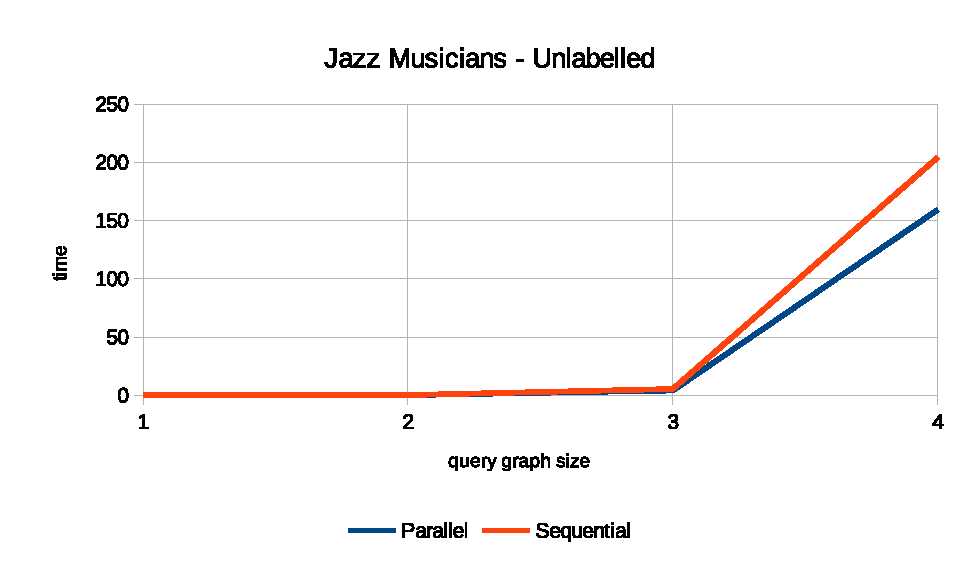
\includegraphics[scale=0.55]{images/Jazz_unlabelled.eps}
        \caption*{(a) average time vs query graph size}        
    \end{minipage} \hfill  
    \begin{minipage}[b]{.45\textwidth}
        \hspace*{-0.2in}
        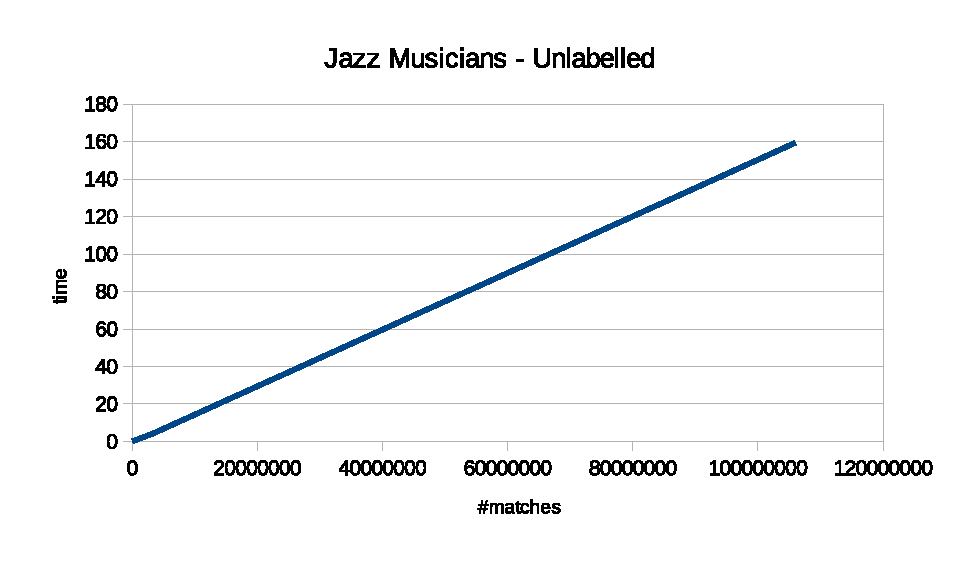
\includegraphics[scale=0.55]{images/Jazz_unlabelled_tpm.eps}
        \caption*{(b) time vs \#matches}       
    \end{minipage}   
\caption{Jazz musicians dataset with unlabelled data and query graphs}
\label{fig:distmx}
\end{figure}

As from the comparison graph in figure 4.1 (a), The parallel implementation runs faster as compared to the sequential version. However, both the implementations take exponential time to get the matches. In figure 4.1 (b), A plot for number of matches vs time elapsed is plotted. The number of matches obtained corresponds to various query graph sizes. We can observe that the time taken per match increases linearly (polynomially).

\begin{figure}[h!]
    \centering
    \begin{minipage}[b]{.45\textwidth}
        \hspace*{-0.5in}
        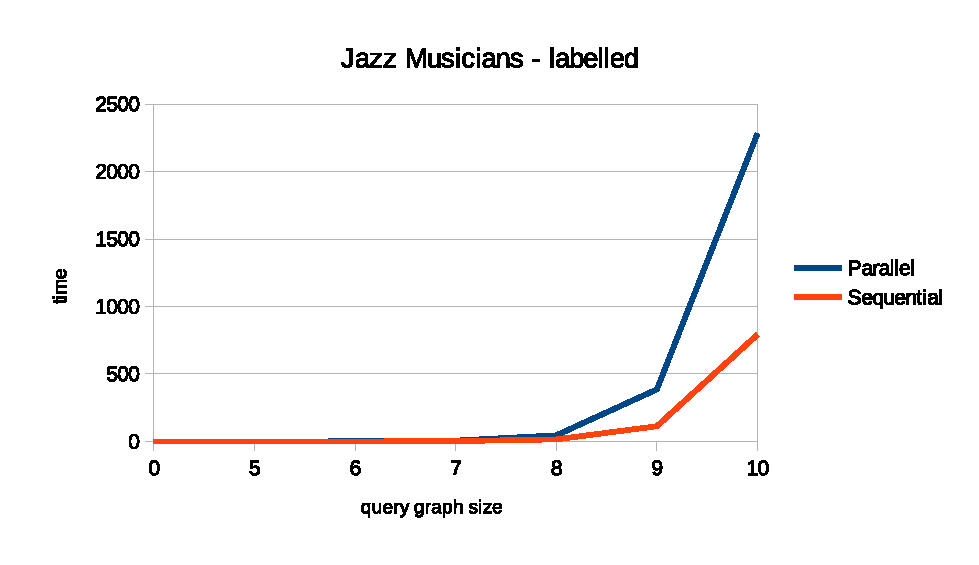
\includegraphics[scale=0.55]{images/Jazz_labelled.eps}
        \caption*{(a) average time vs query graph size}        
    \end{minipage} \hfill  
    \begin{minipage}[b]{.45\textwidth}
        \hspace*{-0.2in}
        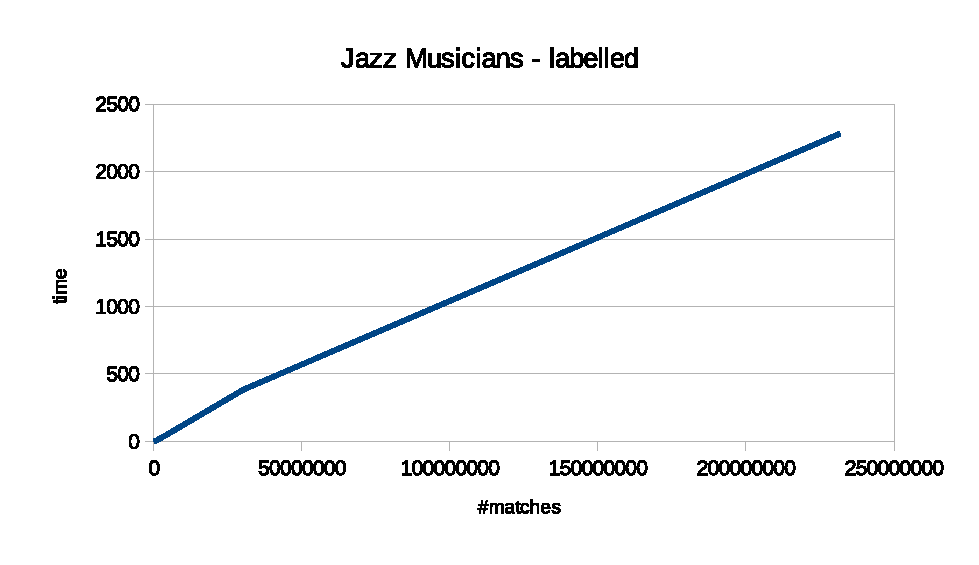
\includegraphics[scale=0.55]{images/Jazz_labelled_tpm.eps}
        \caption*{(b) time vs \#matches}       
    \end{minipage}   
\caption{Jazz musicians dataset with labelled data and query graphs}
\label{fig:distmx}
\end{figure}

For labelled graph, 5 random labels were assigned to the data and the query graphs. In this case, the performance of sequential implementation is better as compared to the parallel implementation. This is because in case of labelled graphs, the number of candidates of each node reduces. Because of which the
number of threads and hence the amount of parallelism decreases.

The algorithms were also compared on labelled data graph and dense labelled query graphs (both with 3 labels). But the result was similar as the sparse query graph.

\begin{figure}[]
\begin{center}
        \centering
        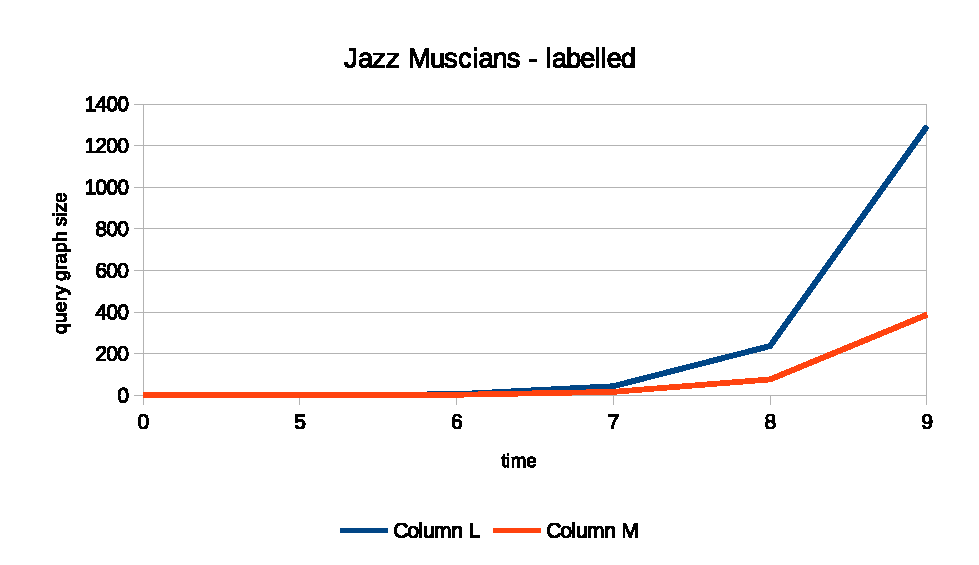
\includegraphics[width=0.7\textwidth]{images/jazz_unlabelled_dense.eps}
        \caption{\textsc{SubgraphSearch}}
        \label{fig:flowchart}
\end{center}
\end{figure}

\section{Dataset: Hamsterster friendships}

Source of this dataset is \cite{hasmtersert}. This graph represents network of friendship between users on the website hamsterster.com. The graph contains 1858 vertices and 12534 edges with a maximum degree of 272 edges and an average degree of 13.492 edges / vertex. Following plot shows the results of parallel and sequential implementation on the unlabelled graph.

\begin{figure}[H]
    \centering
    \begin{minipage}[b]{.45\textwidth}
        \hspace*{-0.5in}
        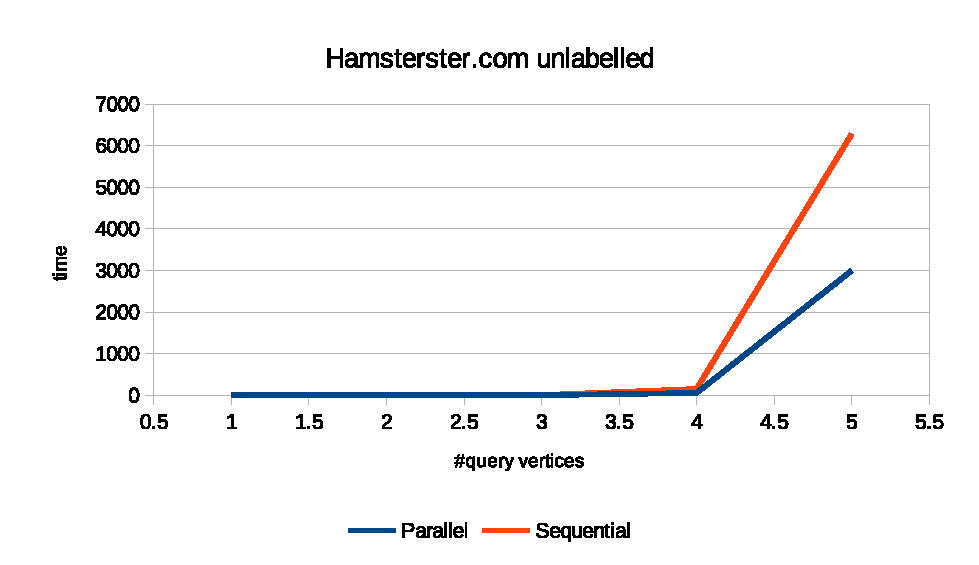
\includegraphics[scale=0.55]{images/hamsterster_unlabelled.eps}
        \caption*{(a) average time vs query graph size}        
    \end{minipage} \hfill  
    \begin{minipage}[b]{.45\textwidth}
        \hspace*{-0.2in}
        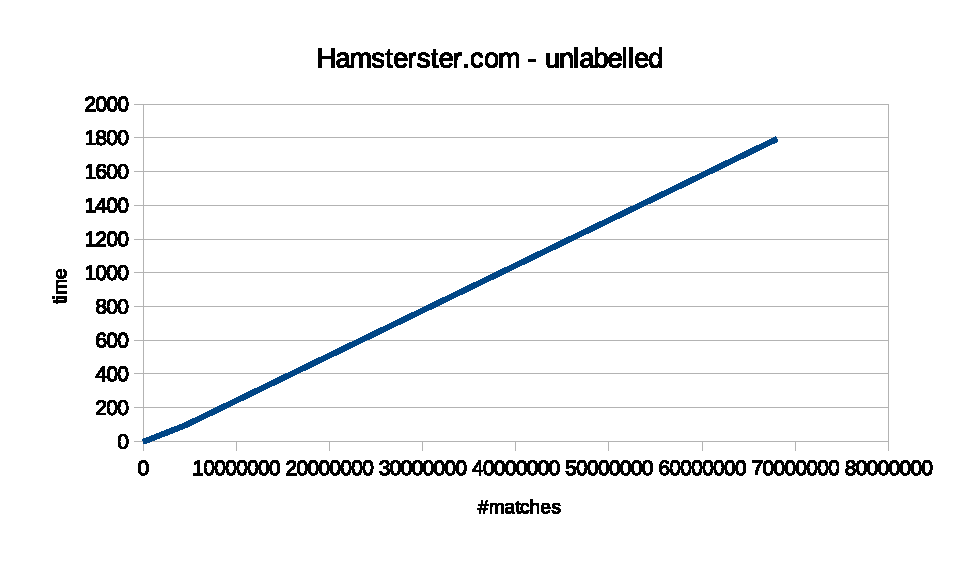
\includegraphics[scale=0.55]{images/hamsterster_unlabelled_tpm.eps}
        \caption*{(b) time vs \#matches}       
    \end{minipage}   
\caption{Hamsterster friendship dataset with unlabelled data and query graphs}
\label{fig:distmx}
\end{figure}

Since this graph is larger as compared to the jazz musicians graph, the number of candidates and hence the number of threads launched is more. Evidently, the performance of the parallel implementation is better than the sequential implementation. Also the average time elapsed per match is again linear.

As for the labelled graphs (5 labels), the performance of both the sequential and parallel versions are similar with the parallel implementation outperforming the sequential implementation for query sizes below 5 vertices.


\begin{figure}[H]
    \centering
    \begin{minipage}[b]{.45\textwidth}
        \hspace*{-0.5in}
        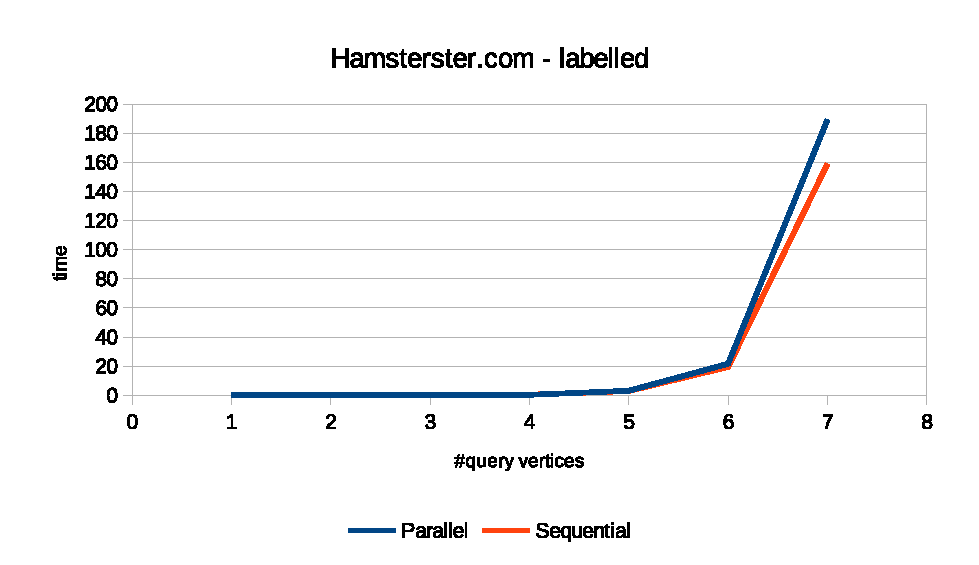
\includegraphics[scale=0.55]{images/hamsterster_labelled.eps}
        \caption*{(a) average time vs query graph size}        
    \end{minipage} \hfill  
    \begin{minipage}[b]{.45\textwidth}
        \hspace*{-0.2in}
        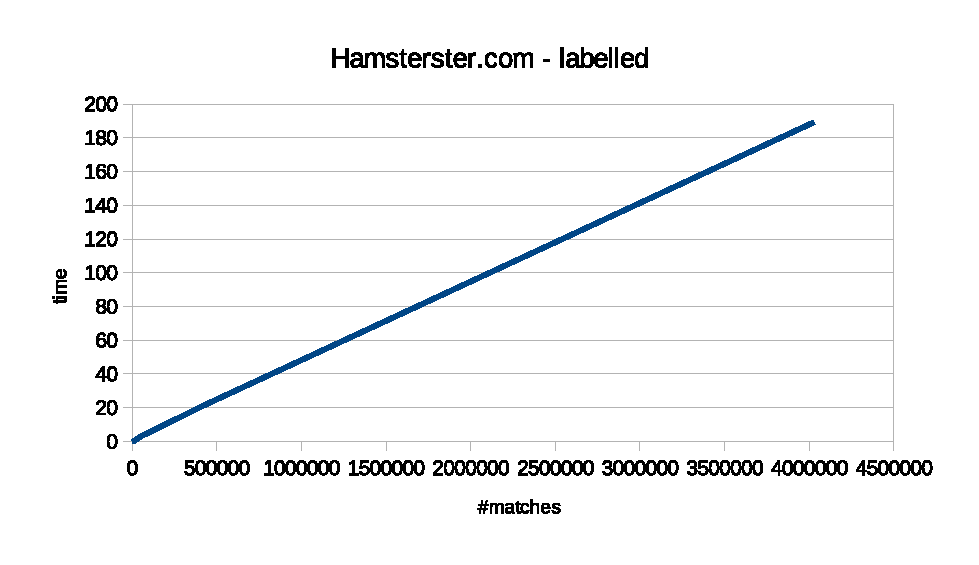
\includegraphics[scale=0.55]{images/hamsterster_labelled_tpm.eps}
        \caption*{(b) time vs \#matches}       
    \end{minipage}   
\caption{Hamsterster friendship dataset with labelled data and query graphs}
\label{fig:distmx}
\end{figure}

\section{Dataset: US power grid}

Source of this dataset is \cite{powergrid}.This dataset contains the contains information on connectivity of the power grid of Western United States. Each node represents either a generator, a transformer or a substation. Each edge of the graph represents a wire connecting either of these. This graphs has 4941 vertices, 6594 edges and the maximum degree of a node is 19 edges. Since this a relatively sparse graph with an average degree of 2.6691 edges / vertex, the query graphs used on this data graph is relatively sparse in order to get sufficient number of matches.

Figure 4.6 (a) shows the comparison between performance of serial and parallel implementation of the algorithms over unlabelled data and query graphs.

\begin{figure}[h!]
    \centering
    \begin{minipage}[b]{.45\textwidth}
        \hspace*{-0.5in}
        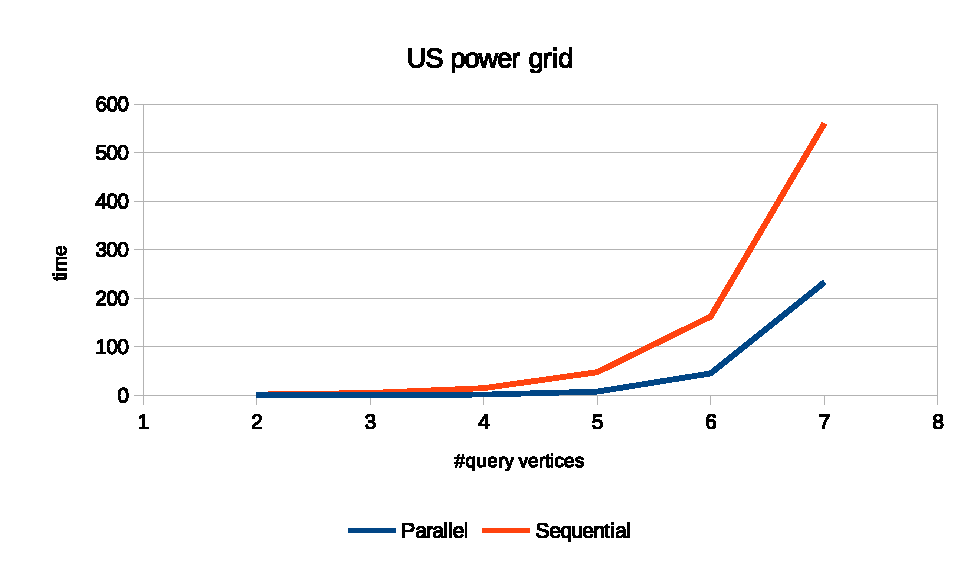
\includegraphics[scale=0.55]{images/USpower_unlabelled.eps}
        \caption*{(a) average time vs query graph size}        
    \end{minipage} \hfill  
    \begin{minipage}[b]{.45\textwidth}
        \hspace*{-0.2in}
        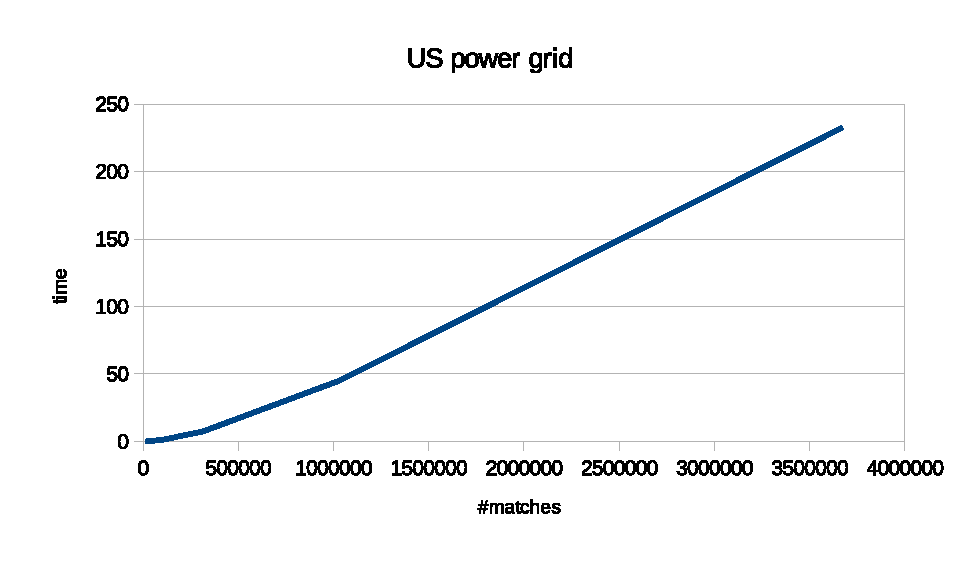
\includegraphics[scale=0.55]{images/USpower_unlabelled_tpm.eps}
        \caption*{(b) time vs \#matches}       
    \end{minipage}   
\caption{US power grid dataset with unlabelled data and query graphs}
\label{fig:distmx}
\end{figure}

The performance of parallel implementation is better as compared to the sequential implementation for this dataset. The number of vertices in this graph is larger than the previous two graphs. The number of threads launched in the execution of parallel version for unlabelled graph is 3715.

Figure 4.7 (a) shows the comparison between performance of serial and parallel implementation of the algorithms over labelled data and query graphs. Since each node in the graph can either be a generator, a transformer or a substation, 3 labels are used for the labelled graph which are randomly assigned to the nodes.

\begin{figure}[h!]
    \centering
    \begin{minipage}[b]{.45\textwidth}
        \hspace*{-0.5in}
        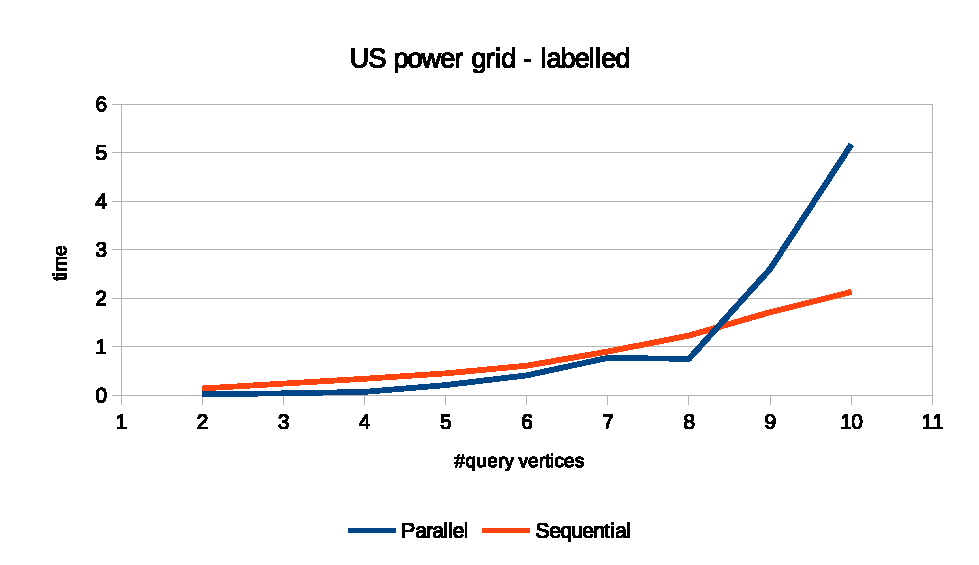
\includegraphics[scale=0.55]{images/USpower_labelled.eps}
        \caption*{(a) average time vs query graph size}        
    \end{minipage} \hfill  
    \begin{minipage}[b]{.45\textwidth}
        \hspace*{-0.2in}
        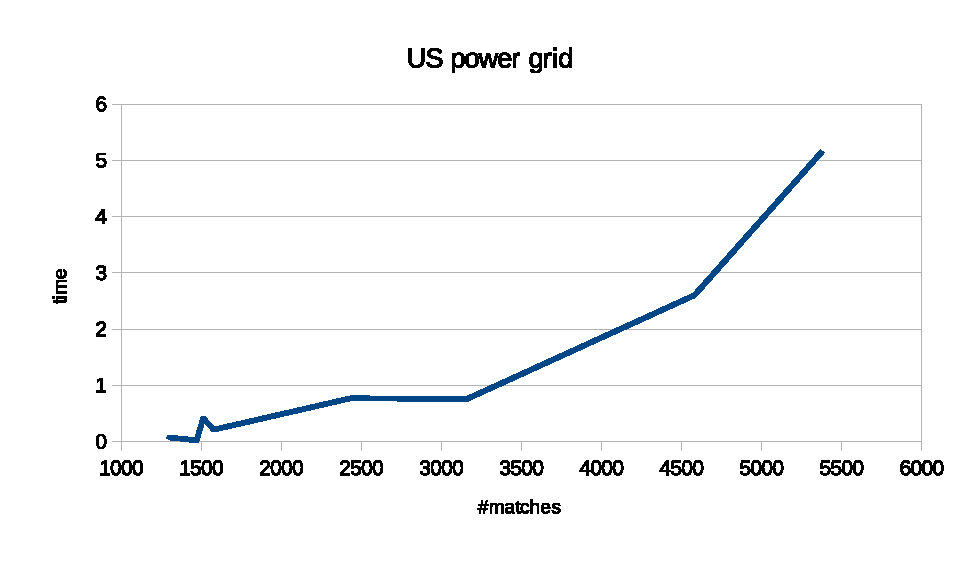
\includegraphics[scale=0.55]{images/USpower_labelled_tpm.eps}
        \caption*{(b) time vs \#matches}       
    \end{minipage}   
\caption{US power grid dataset with labelled data and query graphs}
\label{fig:distmx}
\end{figure}

In the labelled case, the parallel implementation performs better for query graph size $\leq$ 8. This is because, the number of candidates of each node decreases drastically with the increase in size of query vertex (given that data graph is very sparse). Another observation in this case is the irregular time / match curve. This is due to the fact that the number of matches is not monotonically increasing with the increase in query graph size, as was the case with all the previous graphs. The number of matches obtained for query size 2, 3, 4, 5 and 6 were 1472, 1299, 1303, 1580 and 1513 respectively.

\section{Dataset: Chicago Transportation}

Source of this dataset is \cite{chicago}. This graph represents the transportation routes in Chicago city. The vertices in the graph represent a transportation terminal and an edge represents the connection between two terminals. This is a disconnected and a very sparse graph with 1467 vertices, 1298 edges with an average degree of 1.7696 edges / vertex and a max degree of 12 edges.

For this data graph, very sparse query graphs were used because the less number of matches with dense graphs (mostly 0). The comparison of performance is shown in figure 4.8

\begin{figure}[h!]
    \centering
    \begin{minipage}[b]{.45\textwidth}
        \hspace*{-0.5in}
        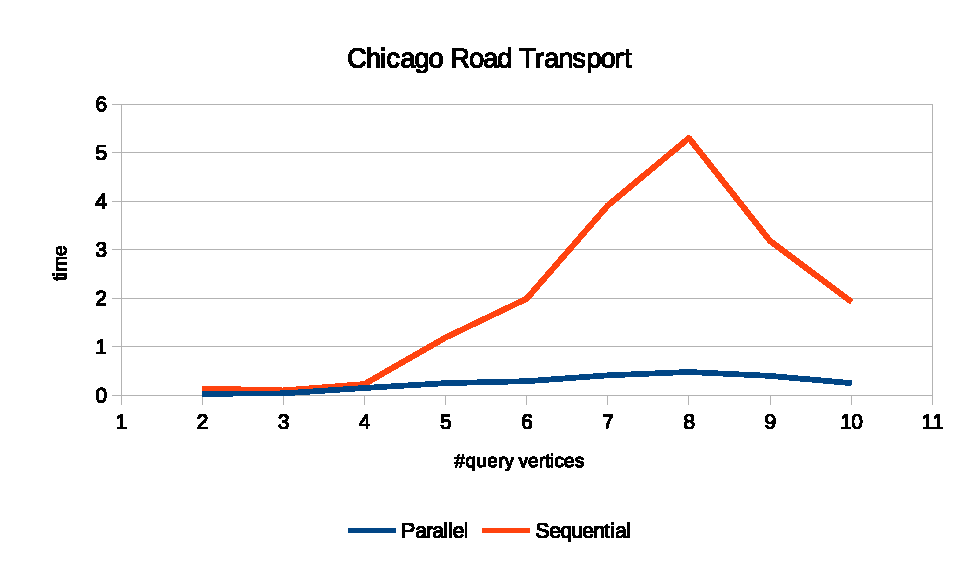
\includegraphics[scale=0.55]{images/chicago_unlabelled.eps}
        \caption*{(a) average time vs query graph size}        
    \end{minipage} \hfill  
    \begin{minipage}[b]{.45\textwidth}
        \hspace*{-0.2in}
        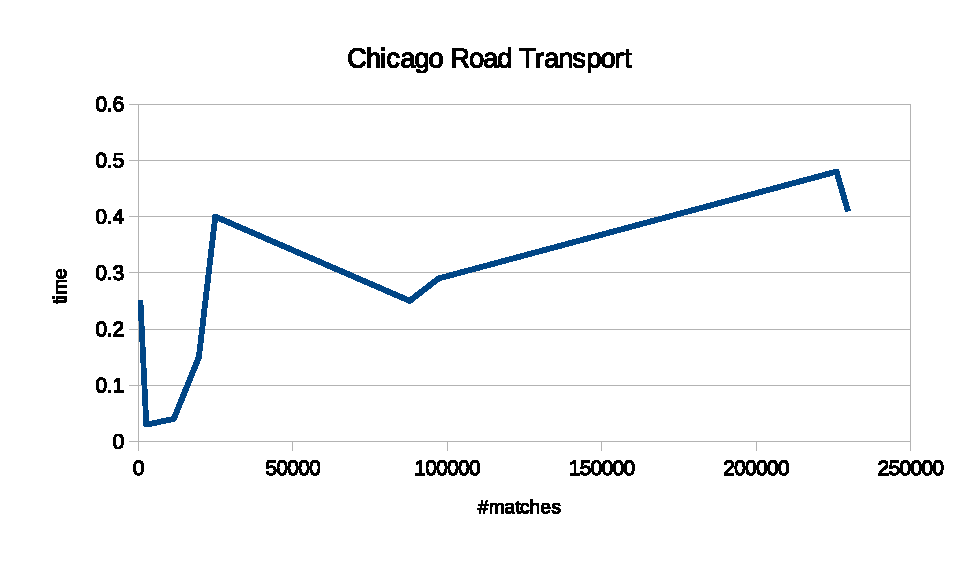
\includegraphics[scale=0.55]{images/chicago_unlabelled_tpm.eps}
        \caption*{(b) time vs \#matches}       
    \end{minipage}   
\caption{Chicago transportation dataset with labelled data and query graphs}
\label{fig:distmx}
\end{figure}

Similar to the US power grid dataset, the time / match curve of this graph is very irregular because of the non monotonocity of the number of matches. For query size 2 to 10 in order, the number of matches are 2596, 11485, 19614, 87886, 97232, 229762, 226072, 24922 and 704. It is evident that the execution time of both the sequential and parallel algorithm depends on the number of matches. However, the parallel implementation outperforms the sequential implementation because of the comparatively large graph size.
\include{parts/chapters/unsupervised}
\chapter{CONCLUSION AND FUTURE WORK}
\label{chap:concl}

The parallel implementation of subgraph isomorphism outperforms the sequential implementation with the increase in size of data graph. As observed from the experiment, the parallel algorithm did not perform very well on small graphs like Hamsterster friendship and Jazz musicians. This is because the number of candidates and hence the number of threads launched were fewer. However, the parallel algorithm did perform well in larger, especially sparse datasets such as Chicago Transportation and the US power grid.

In future, further optimizations can be made to the parallel implementation such as load balancing between threads, to improve the performance even further. More complex heuristics can be developed in order to reduce the number of redundant matches that occur due to rotation and flipping of the same graph.

%%%%%%%%%%%%%%%%%%%%%%%%%%%%%%%%%%%%%%%%%%%%%%%%%%%%%%%%%%%%
% Appendices.
%\include{parts/python-dnn}
%%%%%%%%%%%%%%%%%%%%%%%%%%%%%%%%%%%%%%%%%%%%%%%%%%%%%%%%%%%%
% Bibliography.
\nocite{*}
\pagebreak
\begin{singlespace}
  \begin{small}
	\bibliography{refs}
  \end{small}
\end{singlespace}

%%%%%%%%%%%%%%%%%%%%%%%%%%%%%%%%%%%%%%%%%%%%%%%%%%%%%%%%%%%%

\end{document}
